\section{Results and Discussion}
\label{sec:results}
We first provide the results of the case study. Then we give more general results about the application of conflict-measuring methods to multiple multi-objective systems.

\subsection{Case Study Results}
We parameterized and solved the multi-objective model (\eqref{eqn:objFire}-\eqref{eqn:constraintNonNeg}) for each of the climate scenarios, generating three efficient frontiers: $Z_{\text{None}}$, $Z_{E45}$, and $Z_{E85}$ for the None, Ensemble RCP 4.5, and Ensemble RCP 8.5 scenarios, respectively. Summary details for each frontier are shown in Table \ref{tab:frontiersSummary}, and the frontiers are shown in Figure \ref{fig:frontiersAll}.

\begin{table}[]
\centering
\caption[Summary of efficient frontiers]{Summary of the performance of the efficient frontiers for each climate change scenario.}
\label{tab:frontiersSummary}
\begin{tabular}{ll|lll}
\multicolumn{2}{l|}{}                             & \textbf{None} & \textbf{E45} & \textbf{E85} \\ \hline
\multicolumn{2}{l|}{\textbf{Hypervolume}}         & 0.876977      & 0.866857     & 0.829541     \\ \hline
\multirow{2}{*}{\textbf{Fire hazard}}       & min & 21321.21      & 23219.82     & 23268.02     \\
                                            & max & 21933.29      & 23973.79     & 23724.98     \\ \hline
\multirow{2}{*}{\textbf{NSO habitat}}       & min & 2532.33       & 2412.18      & 2171.10      \\
                                            & max & 2540.05       & 2477.18      & 2481.01      \\ \hline
\multirow{2}{*}{\textbf{Sediment delivery}} & min & 0             & 0            & 0            \\
                                            & max & 24.57         & 63.43        & 69.68        \\ \hline
\multicolumn{2}{l|}{\textbf{Number of solutions}} & 51            & 701          & 1083        
\end{tabular}
\end{table}


\begin{figure}[ht!]
  \subfloat[None]{%
    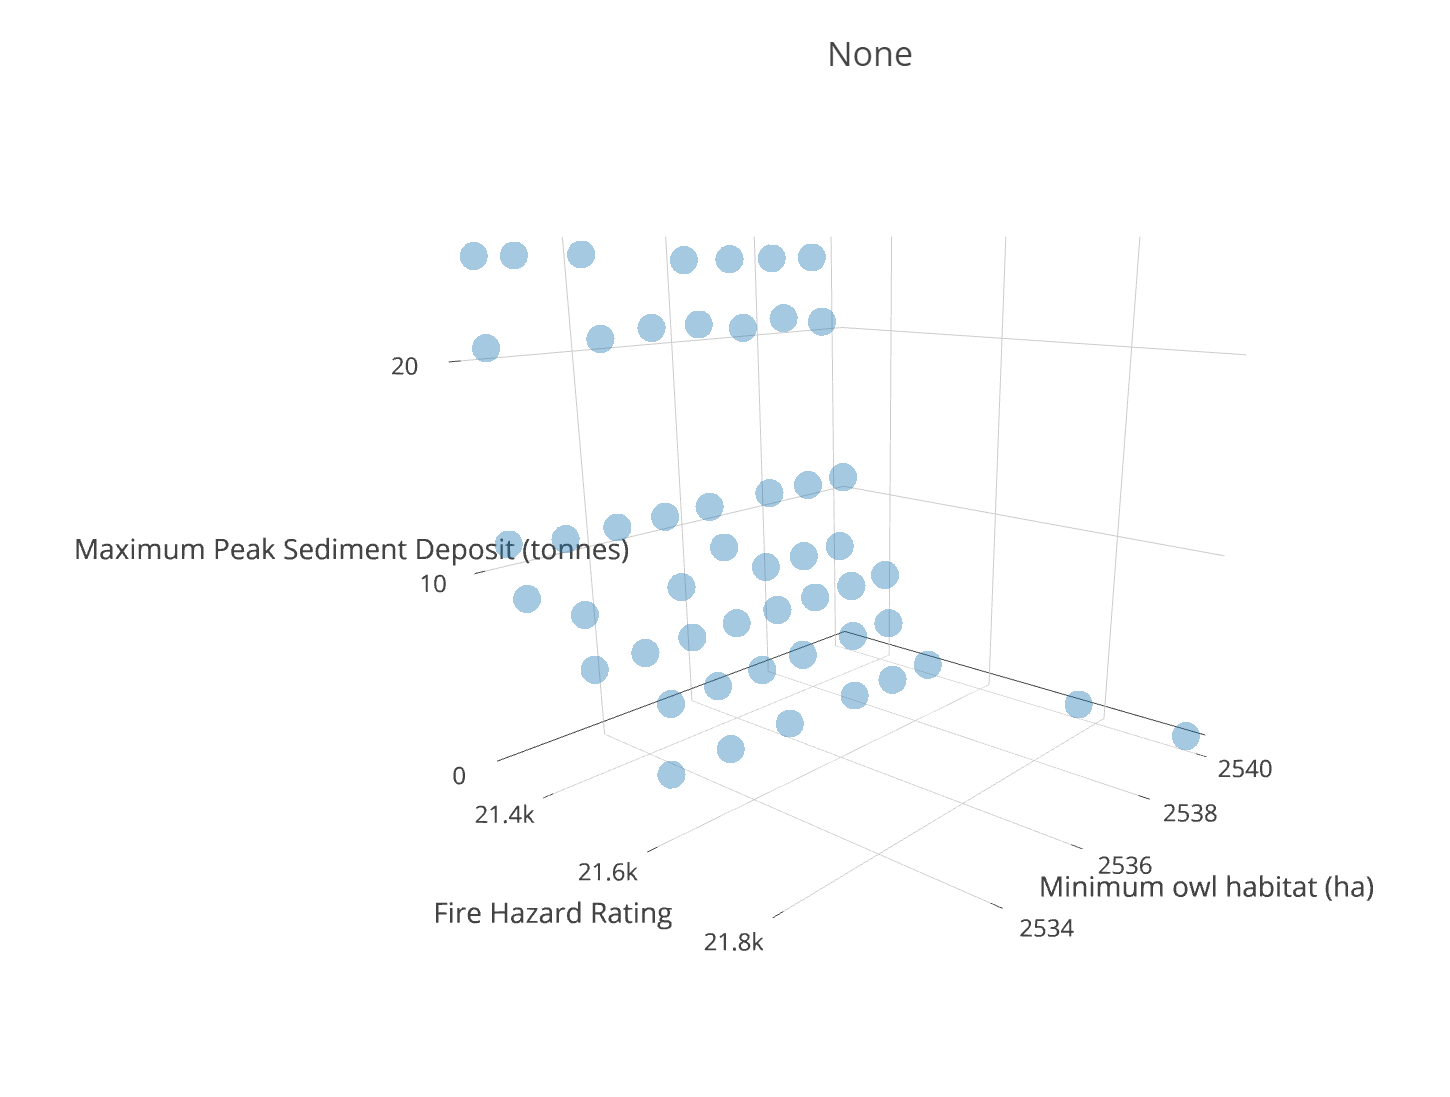
\includegraphics[width=.33\textwidth]{../images/Frontier_None}%
    \label{fig:frontierNone}%
  }\hfill
  \subfloat[Ensemble RCP 4.5]{%
    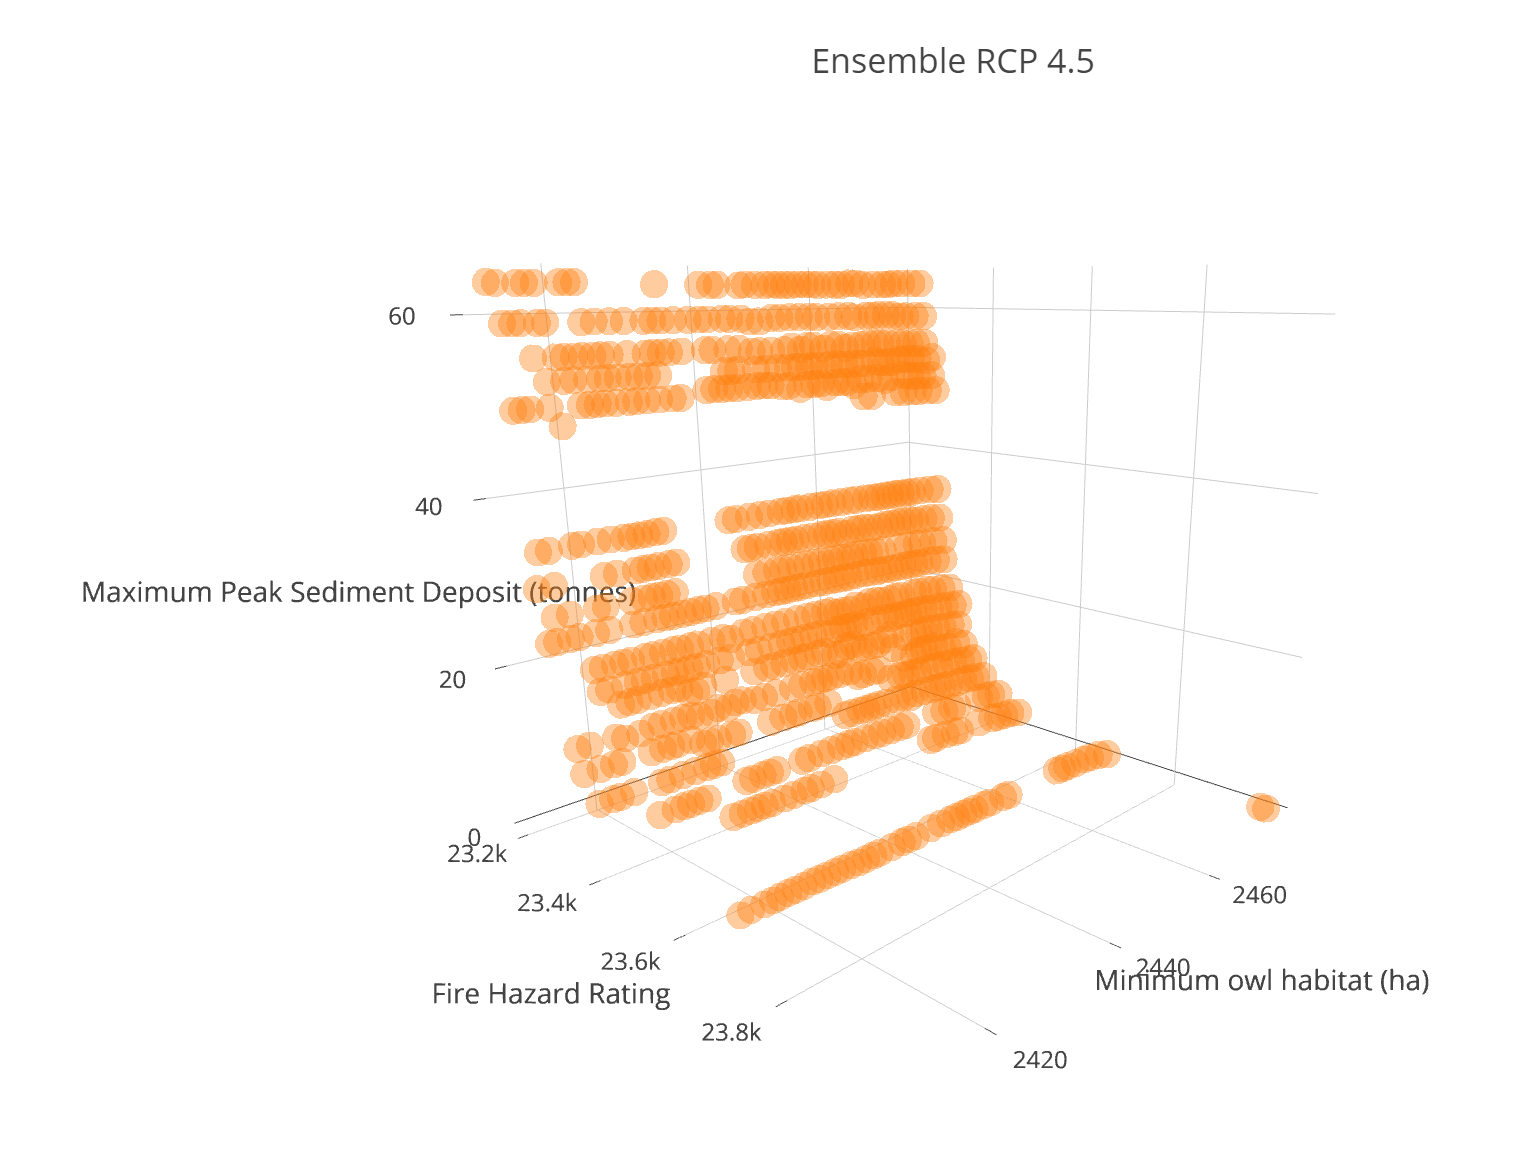
\includegraphics[width=.33\textwidth]{../images/Frontier_E45}%
    \label{fig:frontierE45}%
  }\hfill
  \subfloat[Ensemble RCP 8.5]{%
    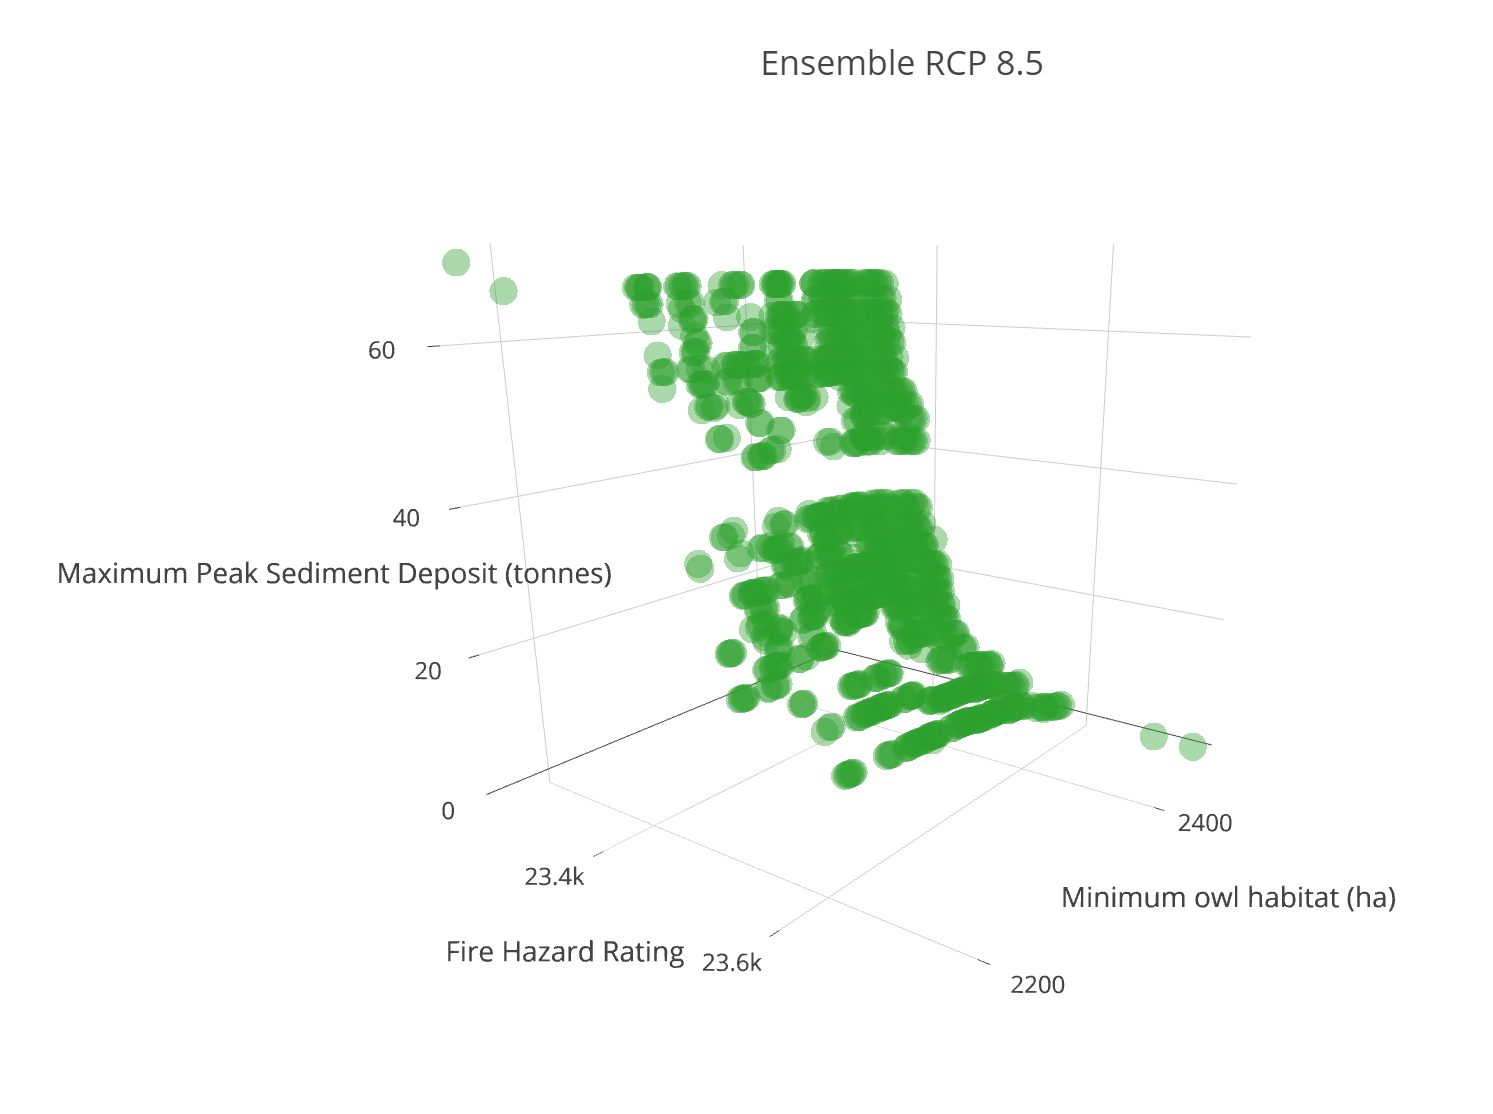
\includegraphics[width=.33\textwidth]{../images/Frontier_E85}%
    \label{fig:frontierE85}%
  }
  \caption[Frontiers for each climate change scenario]{Efficient frontiers for each climate change scenario.}
  \label{fig:frontiersAll}
\end{figure}


% Talk about sources of conflict in between objectives. Well, the conflict metric is higher for this frontier than for this frontier (graph of cross section). The underlying reason for this is bc the ?sed contrib is higher in this scenario than that scenario? or ?the efficacy of treatments is highest in E85 and on the stands located in the watershed?. Something like that. Look into treatment efficacy on WS stands across the climate scenarios. And the sediment contributions vs climate scenarios